\documentclass[border=8pt]{standalone}
\usepackage{fontspec}
\setmainfont{Carlito}
\usepackage{unicode-math}
\setmathfont{Latin Modern Math}
\usepackage{xcolor}
\usepackage{pgfplots}
\pgfplotsset{compat=1.18}
\usetikzlibrary{positioning}

\definecolor{canvabg}{RGB}{246,244,241}
\pagecolor{canvabg}
\begin{document}
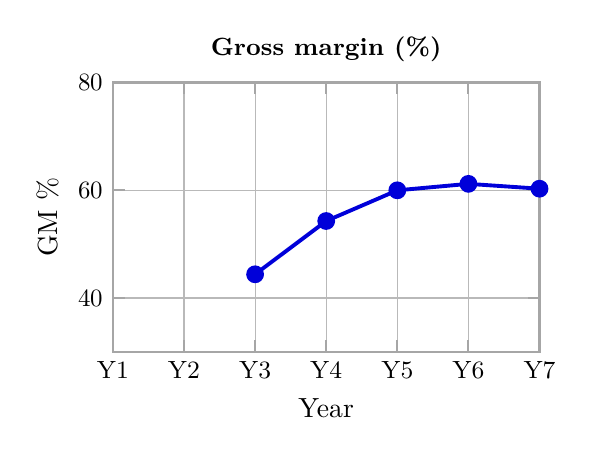
\begin{tikzpicture}
    \begin{axis}[
        width=7cm,
        height=5cm,
        symbolic x coords={Y1,Y2,Y3,Y4,Y5,Y6,Y7},
        xtick=data,
        xlabel={Year},
        grid=major,
        grid style={line width=.3pt, draw=gray!45},
        major grid style={line width=.4pt, draw=gray!55},
        axis line style={line width=0.9pt, draw=gray!70},
        tick style={line width=0.7pt, color=gray!70},
        tick label style={font=\small},
        label style={font=\normalsize},
        title style={font=\small\bfseries, yshift=-2pt},
        legend style={
            font=\scriptsize,
            cells={anchor=west},
            inner sep=2pt,
            row sep=-1pt,
            fill=canvabg,
            draw=gray!50,
        },
        title={Gross margin (\%)},
        ylabel={GM \%},
        ymin=30, ymax=80,
        xmin=Y1, xmax=Y7,
        xtick={Y1,Y2,Y3,Y4,Y5,Y6,Y7},
    ]
    \addplot[line width=1.4pt,blue!85!black,mark=*,mark size=2.5pt,mark options={solid,fill=blue!85!black}]
        coordinates {(Y3,44.4) (Y4,54.3) (Y5,60.0) (Y6,61.2) (Y7,60.3)};
    \end{axis}
\end{tikzpicture}
\end{document}
